\chapter{State of the Art}\label{ch:state-of-the-art}

\section{Problem 1 - Tactile Perception}\label{sec:lit-rev-problem-1}

Based on the contact model categories described in \chapref{ch:modeling}, the most representative was chosen to be \gls{sf} models. 
% since these can provide descriptions of the contact surface shape, and thus enable the solving of the \gls{iep} by deriving surface features for pose estimation. Furthermore, these represent friction forces and moments that is needed to manipulate objects in hand and ensure force closure. 
Within the category of \gls{sf} models, a method fit for this project's use case is to be chosen to solve problem~\ref{prob:1}. \gls{sf} models can furthermore be divided up into three different categories: \gls{aebm}, \gls{efm}, \gls{fem}~\cite{a-modified-elastic-foundation-contact-model-for-application-in-3d-models-of-the-prosthetic-knee} and \gls{ml} models. The different categories can be seen organized in \figref{fig:sf-categories} \medskip
%
\begin{figure}[h]
	\begin{small}
		\begin{center}
			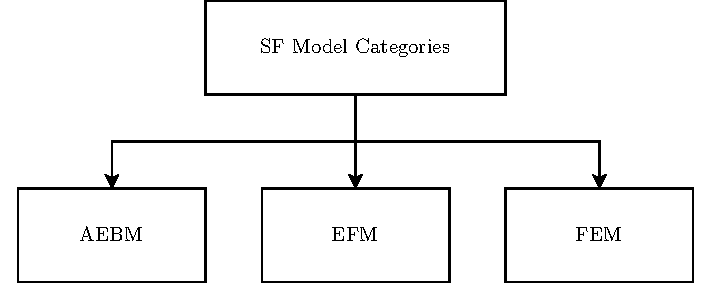
\includegraphics[width=0.8\textwidth]{chapters/state-of-the-art/fig/sf-categories.pdf}
		\end{center}
		\caption{Tree of methods for tactile perception.}
		\label{fig:sf-categories}
	\end{small}
\end{figure}

\gls{aebm} are theoretical formulations of elastic contact areas and the stresses on both the surfaces and the sub-surfaces of the contacting bodies. The first of such models was introduced by Heinrich Rudolf Hertz in \num{1882}~\cite{on-the-contact-of-rigid-elastic-solids-and-on-hardness} and is still used for simple contact cases. In the formulation of the Hertzian contact model, two assumptions are made: Objects in contact are made of linear elastic materials and only small contact deformations occur compared to the dimension of an object. However, robotic \gls{ee} fingertips are often made of non-linear elastic materials and for that reason, the Hertzian contact model does not represent the type of contact in this project~\cite[Chapter 37]{handbook-of-robotics}. To improve on the Hertzian model, a more general formulation can be made which extends the model from linear to nonlinear elastic contacts~\cite{modeling-of-contact-mechanics-and-friction-limit-surfaces-for-soft-fingers-in-robotics-with-experimental-results, the-haptic-and-perceptional-characteristics-of-an-anthropomorphic-curved-soft-finger-structure}. This power-law formulation subsumes the Hertzian contact theory while assuming a circular contact area. Other models have been purposed that combine the descriptions of both friction-contact and the shear-torsion as experienced by the bodies~\cite{the-sliding-of-robot-fingers-under-combined-torsion-and-shear-loading}. \medskip

However, to more accurately describe the contacts involving robot fingers, viscoelastic soft contact model appear more relevant due to such fingers often being made of materials that show viscoelastic properties e.g., rubber, silicone and polymers. Simple models such as  Kelvin-Voigt's~\cite{viscoelasticity} and Maxwell's~\cite{on-the-dynamical-theory-of-gases} models describe the interaction between strain and stress as a spring-damper system in a serial or in a parallel configuration respectively. Models which expand on this idea describe the reacting force as the product of the temporal and the elastic response while incorporating previous stress responses~\cite{mechanical-properties-and-active-remodeling-of-blood-vessels}. To simplify this formulation alternatives have been developed to assume no past stress~\cite{modeling-of-viscoelastic-contacts-and-evolution-of-limit-surface-for-robotic-contact-interface, characteristics-of-contact-and-limit-surface-for-viscoelastic-fingers, effect-of-layer-compliance-on-frictional-behavior-of-soft-robotic-fingers}. Upon these, more modern techniques have been developed which have seen use in similar use cases as the ones of interest in this project. 
% AEBM modern method 2 - A new algorithm for computing the indentation of a rigid body - reformulate - are frictionless MIM (matrix inversion).
One method attempts to expand the description of contacts between rigid indentors and elastic half-spaces, using the \gls{mim} as introduced by Kalker~\cite{on-the-contact-problem-in-elastostatics}, to viscoelastic half-spaces as well. Assuming the surfaces are frictionless, the relationship is described in terms of the pressure distribution, the resultant force on the indenter and the penetration~\cite{a-new-algorithm-for-computing-the-indentation-of-a-rigid-body-of-arbitrary-shape-on-a-viscoelastic-half-space}.
% AEBM modern method 3 - BC's Formulation
Attempts involving solutions to Boussinesq's problem for polynomial pressures acting over polygonal domains~\cite{a-general-approach-to-the-solution-of-boussinesqs-problem-for-polynomial-pressures-acting-over-polygonal-domains} have also been developed and modernized by combining it with Cerruti's solution~\cite{a-boussinesq-cerruti-solution-set-for-constant-and-linear-distribution-of-normal-and-tangential-load-over-a-triangular-area}. However due to numerical singularities being present, modifications are made to threshold the model. For a more complete description without singularities, Love's formulation has been added leading to a more accurate analytical representation but with the cost of an increased computational complexity~\cite{contact-modelling-and-tactile-data-processing-for-robot-skins}. For these Boussinesq-based approaches to be representative two assumptions are made 1) There exists a linear relationship between stress and strain, referred to as deformation, and 2) strains are infinitesimal~\cite[Chapter 6]{the-linearized-theory-of-elasticity}. \medskip

\gls{efm} are methods developed to build upon \gls{aebm} by allowing a simple discrete contact calculation in more general surface geometries. Here the deformable part of the contact is modeled as a layer over a rigid base with a series of discrete and independent springs in the contact normal. A widely used example of this method is Winkler's elastic foundation model~\cite{kl-johnson-and-contact-mechanics}, which has been used in structural engineering for modeling different properties of beams such as stability~\cite{stability-of-a-timoshenko-beam-resting-on-a-winkler-elastic-foundation}, vibrations and buckling~\cite{vibrations-and-buckling-of-a-beam-on-a-variable-winkler-elastic-foundation}. Other \gls{efm} methods have shown accurate modeling performance when applied within the field of medical engineering. Here a comparative study between \gls{aebm}, \gls{efm} and \gls{fem} demonstrate the suggested modified \gls{efm} performs better than the alternatives in 3D knee models when predicting prosthetic knee performance~\cite{a-modified-elastic-foundation-contact-model-for-application-in-3d-models-of-the-prosthetic-knee}. A different method attempts to attain vivo contact pressure predictions for improved knee replacement designs~\cite{experimental-evaluation-of-an-elastic-foundation-model-to-predict-contact-pressures-in-knee-replacements} Within the field of robotics \gls{efm} have provided solutions to problems such as slip~\cite{the-sliding-of-robot-fingers-under-combined-torsion-and-shear-loading}, compliance, sliding~\cite{quasistatic-manipulation-with-compliance-and-sliding, practical-force-motion-models-for-sliding-manipulation}, stiffness and contact mechanics~\cite{stiffness-and-contact-mechanics-for-soft-fingers-in-grasping-and-manipulation} of anthropomorphic grippers. One such method derives friction constraints based on general expressions for non-planar contacts of elastic bodies, where the local geometry and structure of the objects in contact are taken into account. Using these, a linear complementary problem is formulated and solved, resulting in the normal and frictional forces applied at each contact, as well as the relative velocity of the bodies involved~\cite{soft-finger-model-with-adaptive-contact-geometry-for-grasping-and-manipulation-tasks}. \medskip

\gls{fem} are popular general tools for solving PDE~\cite{history-of-finite-element-method:-a-review} and have seen contact applications in a wide range of engineering disciplines due to the assumptions made in \gls{aebm} and \gls{efm} not being applicable in these cases. A great number of these cases exist within the manufacturing industry~\cite{examples-of-fem-application-in-manufacturing-technology} whereas one example is the metal forming processes. Specifically, the estimation of wheel-rail profiles~\cite{contact-mechanics-analysis-of-measured-wheel-rail-profiles-using-the-finite-element-method} has been addressed using \gls{fem} due to the estimation of contacts over a greater surface is needed than what is assumed in \gls{aebm} and \gls{efm}. Other applications such as quality control through sliding wear estimation~\cite{simulating-sliding-wear-with-finite-element-method}, analysis of the responses of fully coupled thermo-elasto-plastic solids in contact~\cite{a-finite-element-procedure-for-the-analysis-of-thermo-mechanical-solids-in-contact} and performing diagnostics of failures in induction motors~\cite{induction-motors-fault-diagnosis-using-finite-element-method:-a-review}. Due to the complexity of modeling the contacts within robotics, \gls{fem} have become a popular choice and enabled tactile applications such as \gls{cobot} tactile skin for ensuring collaborative behavior when in contact~\cite{soft-robot-skin-with-conformal-adaptability-for-on-body-tactile-perception-of-collaborative-robots}, performance estimation of new tactile sensor technologies~\cite{design-and-experimental-research-of-robot-finger-sliding-tactile-sensor-based-on-fbg} and evaluating complex contact types by extending simulations and analysis systems~\cite{grasp-analysis-using-deformable-fingers}.
The modeling complexity has furthermore inspired using \gls{fem} as ground truth results when synthesizing \gls{ml} data in simulations for deep learning models, which has enabled execution speeds \num{75} times greater than simply evaluating \gls{fem}~\cite{sim-to-real-for-robotic-tactile-sensing-via-physics-based-simulation-and-learned-latent-projections, interpreting-and-predicting-tactile-signals-via-a-physics-based-and-data-driven-framework, ground-truth-force-distribution-for-learning-based-tactile-sensing:-a-finite-element-approach}. \medskip

% introduction of ml methods %%%%%%%%%%%%%%%%%%%%%%%%%

The use of these \gls{ml} models has enabled realistic simulations of tactile sensor data. Current literature applies \gls{dl}-based approaches to simulate tactile sensor data for various tasks~\cite{more-than-a-feeling-learning-to-grasp-and-regrasp-using-vision-and-touch, single-grasp-object-classification-and-feature-extraction-with-simple-robot-hands-and-tactile-sensors}. For instance, simulating realistic tactile images from simulated contact depth to bridging
the reality gap for vision-based tactile sensing using a diffusion model~\cite{learning-to-read-braille:-bridging-the-tactile-reality-gap-with-diffusion-models}. Similarly, a \gls{cgan} has been used to simulate realistic tactile sensory data for use in tactile tasks~\cite{learning-to-read-braille:-bridging-the-tactile-reality-gap-with-diffusion-models}. Solutions using simple \gls{mlp} have been applied to enable real-time simulated realistic tactile data~\cite{simulation-of-the-syntouch-biotac-sensor}. \medskip

Given the methods presented above, the \gls{aebm} Boussinesq-Cerruti approach is considered along with the \gls{ml} approach with a \gls{mlp} model. \medskip

Although the Boussinesq-Cerruti approach can produce precise tactile data and can be tailored to suit a particular case, it faces certain challenges. The model relies on certain assumptions regarding the materials in contact, including linear deformation and infinitesimal strains. Furthermore, evaluating the model requires complex calculations, such as multidimensional integrals, which significantly increase computation time and hinder real-time performance. In contrast to the transparency offered by the Boussinesq-Cerruti approach, the \gls{mlp} approach is limited by the black-box nature of \gls{dl} models. Despite this drawback, \gls{mlp}s offer several benefits, such as low execution time and high adaptability to complex systems. Due to the high adaptability and option for real-time performance, the \gls{mlp} model presented in~\cite{simulation-of-the-syntouch-biotac-sensor} is chosen to solve the tactile perception problem i.e. problem \ref{prob:1}.

% While the Boussinesq-Cerruti approach can provide high-quality tactile data with the option to modify and tune the model to fit the specific case, challenges arise as the model makes certain assumptions regarding the materials in contact. These assumptions include: the deformation is assumed linear along with the strains being infinitesimal. Additionally, when evaluating the model expensive computations are necessary such as multidimensional integrals, increasing the computation time and inhibiting real-time performance.

% Boussinesq-based approaches
% 	assumptions are not correct, execution time is slow.
% Machine learning 
% 	Due to these algorithms having a low execution time and high adaptability to complex systems
% For these Boussinesq-based approaches to be representative two assumptions are made 1) There exists a linear relationship between stress and strain, referred to as deformation, and 2) strains are infinitesimal

% tactile solutions for NN~\cite{touching-a-nerf-leveraging-neural-radiance-fields-for-tactile-sensory-data-generation}
% biotac_sim example
% One such example is the simulation of the SynTouch BioTac sensor when mounted on a Shadow Dexterous hand~\cite{simulation-of-the-syntouch-biotac-sensor}

% compare analytical and ml methods for pros and cons, choose which method is ideal for this case %%%%%%%%%%%%%%%%


% Due to these algorithms having . One such example is [insert machine learning achievements and how they are used in sensor simulation] \medskip

% Due to the accurate displacement representation and execution time, the machine learning-based approach is chosen.

% The contact model chosen for this project is the \gls{aebm} Love's formulation due to its capabilities of representing contact surface displacements with great precision~\cite{contact-modelling-and-tactile-data-processing-for-robot-skins}.

\section{Problem 2 - Pose Estimation}\label{sec:lit-rev-problem-2}

\gls{pe}, which involves determining the position and orientation of an object in 3D space, has been the subject of many research studies. The literature has identified two main categories of methods for solving this problem: those based on \gls{dl}, and those based on point cloud registration. \medskip

These can along with their subcategories be seen in~\figref{fig:pe-categories} as inspired by~\cite{a-comprehensive-survey-on-point-cloud-registration}.

\begin{figure}[h]
	\begin{small}
		\begin{center}
			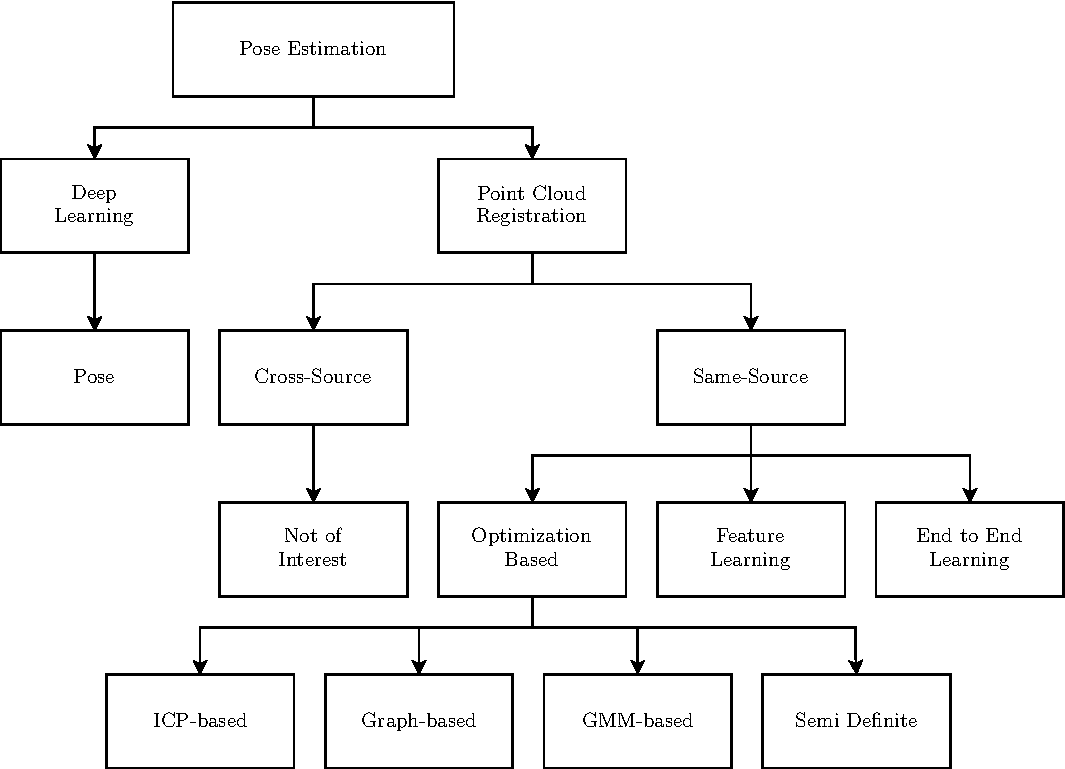
\includegraphics[width=0.8\textwidth]{chapters/state-of-the-art/fig/pe-categories-v3.pdf}
		\end{center}
		\caption{Tree of methods for solving the point cloud registration problem. The categorization is inspired by~\cite{a-comprehensive-survey-on-point-cloud-registration}.}
		\label{fig:pe-categories}
	\end{small}
\end{figure}

Purely \gls{dl} based methods learn feature representations of input data, often in the form of images, and use them to estimate the subject's pose. This is commonly done in the context of human pose estimation~\cite{hands-deep-in-deep-learning-for-hand-pose-estimation, deeppose:-human-pose-estimation-via-deep-neural-networks, deeplabcut:-markerless-pose-estimation-of-user-defined-body-parts-with-deep-learning}. While these methods have shown extensive use in these cases, their applicability in this project is limited and thus excluded from consideration. \medskip

The other method group i.e. \gls{pcr} methods are separated into two subgroups: cross-source and same-source \gls{pc}s. Here cross-source refers to a \gls{pc} produced by combining information from sensors of different kinds e.g. visual- and tactile sensors, while same-source methods only produce \gls{pc}s based on information from the same kind of sensors e.g. only tactile sensors. 
While cross-source approaches have shown utility in an extensive range of applications~\cite{a-systematic-approach-for-cross-source-point-cloud-registration-by-preserving-macro-and-micro-structures,a-coarse-to-fine-algorithm-for-matching-and-registration-in-3d-cross-source-point-clouds,a-comprehensive-survey-on-point-cloud-registration} their applicability in this project is minimal, as purely tactile pose estimation is the problem of interest as presented in \chapref{ch:intro}. \medskip

\gls{pcr} methods from the same source data can be categorized into three sub-categories: end-to-end learning, feature-learning, and optimization-based methods. End-to-end learning-based methods use a neural network to estimate the transformation matrix that aligns two point clouds. Proposed solutions include using neural networks for scene completion to estimate the relative pose between RGB-D scans~\cite{extreme-relative-pose-estimation-for-rgb-d-scans-via-scene-completion}, learning registration patterns as parametric functions through a scan completion module and pairwise matching module~\cite{non-rigid-point-set-registration-networks}, and a fast feature-metric point cloud registration framework to minimize the feature-metric projection error without correspondences~\cite{feature-metric-registration:-a-fast-semi-supervised-approach-for-robust-point-cloud-registration-without-correspondences}.\medskip

In contrast, feature-learning methods use deep neural networks to learn robust feature correspondence searches, which are then used in estimation algorithms such as \gls{ransac}. In the literature, models have been developed to extract local geometric descriptors from RGB-D reconstructions~\cite{3dmatch:-learning-local-geometric-descriptors-from-rgb-d-reconstructions}, to learn globally informed 3D local feature descriptors~\cite{ppfnet:-global-context-aware-local-features-for-robust-3d-point-matching}, and to use siamese deep learning architectures with convolutional layers through a voxelized smoothed density value (SDV) representation~\cite{the-perfect-match:-3d-point-cloud-matching-with-smoothed-densities}. \medskip

% icp based methods
% In this paper we combine the Iterative Closest Point (ICP) and point-to-plane ICP algorithms into a single | Generalized-ICP algorithm

% 3 icp algorithm solutions


% 3 graph-based solutions 

% 3 gmm-methods

% semi-definite programming

% RCQP
% This allowed us to solve the original non-convex problem in a global fashion using its connection to the convex relaxation through duality theory


% we add GNC for robust outlier rejection

Lastly, registration methods based on optimization are employed to estimate the transformation matrix through two stages: correspondence searching and transformation estimation. Their goal is to minimize a cost function that gauges the dissimilarity between two point clouds. Within this category, there are four sub-categories identified: \gls{icp}-based, graph-based, \gls{gmm}-based, and semi-definite programming-based methods. \medskip

Since the original proposal in 1992~\cite{a-method-for-registration-of-3-d-shapes} using point-to-point correspondences, \gls{icp}-based methods have evolved and incorporated different types of correspondences to improve performance. Examples include point-to-plane~\cite{object-modelling-by-registration-of-multiple-range-images} and plane-to-plane~\cite{generalized-icp}. Modern approaches also employ complementary methods such as point cloud filtering, adaptive fireworks algorithms, and KD-Trees~\cite{improved-iterative-closest-point-icp-3d-point-cloud-registration-algorithm-based-on-point-cloud-filtering-and-adaptive-fireworks-for-coarse-registration}. \medskip

% graph-based approaches 
The main idea of graph-based registration methods is to use a non-parametric model~\cite{a-review-of-point-set-registration:-from-pairwise-registration-to-groupwise-registration}. In this method, correspondences between two graphs are found by considering both the vertices and edges, making it an optimization problem~\cite{a-review-of-point-set-registration:-from-pairwise-registration-to-groupwise-registration}. To solve this optimization problem, there are two categories of graph-matching methods based on the objective functions' constraints: second-order and high-order methods~\cite{the-graph-matching-problem}. Second-order methods include \gls{csgm}~\cite{a-systematic-approach-for-cross-source-point-cloud-registration-by-preserving-macro-and-micro-structures}, which uses a linear program to solve the graph-matching problem and apply it to solve the cross-source point cloud registration task, \gls{fgm}~\cite{factorized-graph-matching} factorizes the large pairwise affinity matrix into smaller matrices and solves the graph-matching problem with a simple path-following optimization algorithm. Spectral graph~\cite{a-spectral-technique-for-correspondence-problems-using-pairwise-constraints} uses a spectral relaxation method to approximate the \gls{qap}, and \gls{sdp} relaxation is used to relax the non-convex constraint using a convex semi-definite. While higher-order graph matching provide methods for~\cite{probabilistic-graph-and-hypergraph-matching} design a probabilistic approach to solve the high-order graph-matching problem, while~\cite{a-tensor-based-algorithm-for-high-order-graph-matching} design a triangle similarity and convert the graph-matching problem into a tensor optimization problem. More recent work, such as~\cite{elastic-net-constraint-based-tensor-model-for-high-order-graph-matching} suggests an elastic net to control the trade-off between the sparsity and accuracy of the matching results by incorporating the Elastic-Net constraint into the tensor-based graph matching mode. \medskip

% gaussian mixture model
% \gls{gmm}-based methods attempt to convert the registration problem into a likelihood maximization problem for the input data, leading to the literature being focused on developing optimization strategies to maximize the likelihood and optimize the transformation matrix. One such example is~\cite{information-retrieval-for-music-and-motion} which introduces a \gls{cpd} in the form of a motion drift idea into the GMM framework by imposing constraints on transformation estimation. A different approach can be seen in~\cite{convex-hull-indexed-gaussian-mixture-model-ch-gmm-for-3d-point-set-registration} which combines the GMM with the convex hull, which is a tighter set of the original point set, to reduce computation complexity. Additionally, \gls{jrmpc}~\cite{a-generative-model-for-the-joint-registration-of-multiple-point-sets} approach registration as a clustering problem, where the transformation is optimized by solving the \gls{gmm}. More recently, \gls{deepgmr}~\cite{deepgmr:-learning-latent-gaussian-mixture-models-for-registration} has utilized deep learning to learn the correspondences between \gls{gmm} components and points. This enables the estimation of both the transformation and \gls{gmm} parameters in a single forward step.

\gls{gmm}-based methods commonly tackle the point cloud registration problem by transforming it into a likelihood maximization problem for the input data. This has resulted in the development of several optimization strategies aimed at maximizing the likelihood and optimizing the transformation matrix. For instance, a motion drift idea was introduced into the \gls{gmm} framework by~\cite{information-retrieval-for-music-and-motion} in the form of \gls{cpd} which imposes constraints on transformation estimation. In another approach,\cite{convex-hull-indexed-gaussian-mixture-model-ch-gmm-for-3d-point-set-registration} combines \gls{gmm} with the convex hull to reduce computation complexity. Furthermore, \gls{jrmpc}~\cite{a-generative-model-for-the-joint-registration-of-multiple-point-sets} cast registration as a clustering problem where the transformation is optimized by solving the \gls{gmm}. Recently, \gls{deepgmr}~\cite{deepgmr:-learning-latent-gaussian-mixture-models-for-registration} employed \gls{dl} to learn the correspondences between \gls{gmm} components and points, enabling the estimation of both the transformation and \gls{gmm} parameters in a single forward step. \medskip

Lastly, within semidefinite programming different optimization groups exist, such as \gls{socp}, \gls{qp} and \gls{qcqp}. Due to the subject of interest being a rotation in SO(\num{3}), the constraints of the rotation matrix, i.e. quadratic constraints, must be respected. Because of this, the methods of \gls{qcqp} are of interest. \medskip
One such example provides estimates which are insensitive to a large fraction of spurious correspondences through decoupling the scale, rotation, and translation estimation. This decoupling enables the solving of these in cascade for the three transformations. The method is referred to as TEASER (Truncated least squares Estimation And SEmidefinite Relaxation), which solve large \gls{sdp} relaxations, and additionally comes with a second fast and certifiable algorithm, named TEASER++. To decrease execution time this method uses \gls{gnc} to solve the rotation subproblem and applies Douglas-Rachford Splitting to enable efficiently certify global optimality~\cite{teaser:-fast-and-certifiable-point-cloud-registration}. Secondly, Invariant-based Highly Robust Point Cloud Registration (IRON) applies a similar methodology as to TEASER, but instead applies RANSIC (RANdom Samples with Invariant Compatibility) to robustly estimates the scale between two sets of point clouds~\cite{iron:-invariant-based-highly-robust-point-cloud-registration}. Finally, \gls{rcqp} formulates a \gls{qcqp} problem with a full set of quadratic rotational constraints and obtains a Lagrangian dual relaxation, which empirically recovered a globally optimal solution in \SI{100}{\percent} of the tested cases, although why strong relaxation seems to hold has yet to be shown~\cite{convex-global-3d-registration-with-lagrangian-duality}. \medskip

Among the categories presented above, the ones of particular interest are optimization-based techniques due to their mature mathematical foundation and possible certifiable optimality and outlier rejection capabilities, and \gls{dl}-based techniques due to their adaptability and low execution time. While \gls{dl}-based methods can learn feature representations of point clouds and estimate the transformation between two point clouds, optimization-based approaches with outlier rejection can effectively handle noise and outliers in the data, which is a common problem within the \gls{pcr} problem. Due to this, the chosen method is the optimization based \gls{rcqp} method with \gls{gnc} outlier rejection~\cite{graduated-non-convexity-for-robust-spatial-perception:-from-non-minimal-solvers-to-global-outlier-rejection}.


% %&&&&&&&&&&&&&&&&&&&&&&&&&&&
% intro -system setup - sota - model  prob 1 ...
% kalman filter - gnc is sensor abstracttion level
% expand on list of thesis overviewz
% 


% %&&&&&&&&&&&&&&&&&&&&&&&&&&&



% Recently, more sophisticated SDP-based methods have been proposed to solve the registration problem. For instance, Gao et al. [5] proposed an efficient global registration algorithm based on a pairwise comparison of points in point clouds, where SDP is used to optimize the matching problem. This method performs well on point clouds with both small and large overlaps.

% Another SDP-based method that has been proposed is the Sparse Correlation Assignment and Matching (SCAM) method by Li et al. [6]. SCAM is an efficient method that can handle large-scale registration problems. It involves solving an SDP problem using a weighted nuclear norm penalty function. The method has been shown to be robust to noise and outliers, and it outperforms traditional methods like ICP and coherent point drift (CPD) [7] in terms of accuracy and efficiency.

% In addition to SDP-based registration methods, other graph-based methods have also shown promising results. For example, the Fast Approximate Nearest-Neighbor Graph (FANNG) method proposed by Li et al. [8] constructs a graph structure to find approximate nearest neighbors between two point clouds. The graph is then optimized using an SDP algorithm to obtain accurate correspondences. Another graph-based method is the pairwise geometric matching (PGM) method proposed by Wang et al. [9], which uses an SDP relaxation to solve the 
% geometric matching problem between two point clouds.


% A final example is the RCQP


% read RCQP paper along with 2103.02690.pdf

% semidefinite programming

% The positive semi-definite properties of the graph Laplacian make it suitable for solving the point set registration problem using semi-definite relaxation. An example of this approach is PSR-SDP [44], which has been applied to multiple point sets registration. Teaser [105], on the other hand, uses graduated non-convexity to solve the rotation sub-problem. This method employs Douglas-Rachford Splitting to efficiently certify global optimality, thus mitigating the high computational cost of SDP relaxation. However, Teaser may still suffer from local minima. To overcome this issue, OPRASANC [58] introduces a graduated optimization strategy that achieves better efficiency than Teaser. 

% Although semi-definite relaxation achieves the global minimum of the original problem, it faces scalability issues [47] and can only handle up to 15 points [53]. To address this, some techniques have been proposed. For example, [53] uses Markov random field techniques to approximate the linear programming relaxation solution, while PM-SDP [67] reduces the dimension of semi-definite constraints to improve efficiency. However, these methods are only suitable for middle-sized point cloud registration problems, and scalability remains a topic of ongoing research.

% Canonical Correlation Analysis (CCA) is one such optimization-based approach that seeks to maximize the correlation between two sets of variables. Chen et al. [6] used CCA to compute correspondences between two point clouds and used a closed-form solution to estimate the transformation. 

% However, CCA can be sensitive to noise and outliers. Robust Canonical Correlation Analysis (RCCA) is an extension of CCA that is more robust to outliers and noise. Wang et al. [7] proposed a method that uses RCCA to compute correspondences between two point clouds and a robust quadratic program to estimate the transformation. RCCP, the resulting method, has demonstrated greater robustness to noise and outliers than traditional CCA-based methods. 

% RCQP is another optimization-based approach that is often combined with outlier rejection techniques to handle noise and outliers in the data. Li et al. [11] proposed a robust registration method based on dual geometric constraint and quadratic programming, while Zhang and Ye [13] proposed a robust point cloud registration algorithm based on quadratic programming and gradient descent. 

% The RCQP algorithm with GNC outlier rejection has also shown promising results in point registration.


% Zhou et al. [2] introduced Fast Global Registration, which employs a neural network to compute correspondences between two point clouds, followed by a closed-form solution for the transformation estimation.

% The point registration problem is a challenging task in computer vision and robotics, which involves finding the transformation that aligns two point clouds acquired from the same sensor. In recent years, deep learning-based and optimization-based approaches have shown great potential in solving this problem.

% Optimization-based approaches, on the other hand, formulate the point registration problem as an optimization problem and seek to minimize a cost function that measures the dissimilarity between the two point clouds. 

% One such approach is Canonical Correlation Analysis (CCA), which seeks to maximize the correlation between two sets of variables. This method has been applied to point registration by Chen et al. [6], who used it to compute the correspondences between two point clouds, and then used a closed-form solution to estimate the transformation.

% Another optimization-based approach is Robust Canonical Correlation Analysis (RCCA), which is an extension of CCA that is more robust to outliers and noise. RCCA has been used for point registration by Wang et al. [7], who proposed a method that uses RCCA to compute the correspondences between two point clouds, and then uses a robust quadratic program to estimate the transformation. This method, called RCCP, was shown to be more robust to noise and outliers than traditional CCA-based methods.

% RCQP is another optimization-based approach that has been used for point registration, particularly in combination with outlier rejection techniques. Li et al. [11] proposed a robust registration method for point clouds based on dual geometric constraint and quadratic programming, which can effectively handle outliers and noise in the data. Zhang and Ye [13] proposed a robust point cloud registration algorithm based on quadratic programming and gradient descent, which can achieve sub-millimeter accuracy in point registration. A Robust and Efficient Registration Method for Point Clouds Based on the RCQP Algorithm with GNC Outlier Rejection [10] is another example of an RCQP-based method with outlier rejection that has demonstrated promising results in point registration.

% In conclusion, both deep learning-based and optimization-based approaches have shown great potential in solving the point registration problem. While deep learning-based methods can learn feature representations of point clouds and estimate the transformation between two point clouds, optimization-based approaches such as CCA, RCCA, and RCQP can formulate the point registration problem as an optimization problem and effectively handle noise and outliers in the data. Future research could focus on combining these different approaches to further improve the accuracy and robustness of point registration.

% References

% Chetverikov, D., & Stepanov, D. (2002). A fast effective algorithm for point set registration. In Proceedings of the IEEE International Conference on Computer Vision (Vol. 2, pp. 1071-1078).

% Besl, P. J., & McKay, N. D. (1992). A method for registration of 3-D shapes. IEEE Transactions on pattern analysis and machine intelligence, 14(2), 239-256.

% Chen, Y., Medioni, G., & Weizman, A. (1992). Object modeling by registration of multiple range images. Image and vision computing, 10(3), 145-155.

% Rusu, R. B., Blodow, N., & Beetz, M. (2009, May). Fast point feature histograms (FPFH) for 3D registration. In 2009 IEEE International Conference on Robotics and Automation (pp. 3212-3217). IEEE.

% Pomerleau, F., Colas, F., & Siegwart, R. (2013). A review of point cloud registration algorithms for mobile robotics. Foundations and Trends® in Robotics, 2(1-2), 1-104.

% Amiri, R., & Rezaei, M. (2019). A review of point cloud registration methods. Journal of Intelligent & Robotic Systems, 93(3-4), 409-446.

% Zhang, C., Zhu, J., Zhang, C., Lu, F., & Liu, Y. (2020). A survey of point cloud registration based on deep learning. IEEE Access, 8, 205788-205813.

% Chen, Y., & Medioni, G. (1991). Object modelling by registration of multiple range images. Image and vision computing, 10(3), 145-155.

% Aiger, D., Shamir, A., & Cohen-Or, D. (2008, August). 3D photography on your desk. In ACM Transactions on Graphics (TOG) (Vol. 27, No. 3, p. 68). ACM.

% Gao, J., Hou, M., Wang, Y., Zhang, X., & Zhao, Q. (2021). A survey of point cloud registration: From classical iterative methods to deep learning-based techniques. Signal Processing: Image Communication, 97, 116358.

% Leordeanu, M., & Hebert, M. (2005). A spectral technique for correspondence problems using pairwise constraints. In Computer Vision, 2005. ICCV 2005. Tenth IEEE International Conference on (Vol. 2, pp. 1482-1489). IEEE.

% Myronenko, A., & Song, X. (2010). Point set registration: Coherent point drift. IEEE Transactions on Pattern Analysis and Machine Intelligence, 32(12), 2262-2275.

% Yang, B., Luo, C., Wu, L., & Zhang, H. (2020). Robust point cloud registration algorithm based on RCQP with GNC outlier rejection. Journal of Visual Communication and Image Representation, 72, 102894.

% Hotelling, H. (1936). Relations between two sets of variates. Biometrika, 28(3/4), 321-377.

% Hardoon, D. R., Szedmak, S., & Shawe-Taylor, J. (


\section{Problem 3 - In-Hand Manipulation}\label{sec:lit-rev-problem-3}

% In-hand manipulation is an important aspect of robotic manipulation that allows robots to grasp and manipulate objects in a more dexterous manner. A key component of in-hand manipulation is the gripper, which must be capable of grasping and manipulating objects with a high degree of precision and adaptability. In recent years, there has been significant research on the development of dexterous grippers for in-hand manipulation. In this literature review, we will survey some of the methods and techniques for performing in-hand manipulation using dexterous grippers.

% One approach to achieving dexterous manipulation is the use of soft robotic grippers. Soft grippers can deform around objects, providing a more adaptive and gentle grasp. In [1], Polygerinos et al. presented a soft robotic gripper that uses a pneumatically actuated elastomer to wrap around and grip objects. The gripper was shown to be capable of grasping a variety of objects and manipulating them in various ways, such as rotating a pencil or turning a key.

% Another approach to dexterous manipulation is the use of multi-fingered robotic hands. Multi-fingered hands have the advantage of being able to grasp objects from different angles and with different forces. In [2], Chalon et al. presented a robotic hand with three fingers that was able to grasp and manipulate objects with a high degree of dexterity. The hand was shown to be capable of performing tasks such as flipping a pancake and grasping small objects.

% One challenge with multi-fingered hands is the complexity of their control. To address this issue, some researchers have explored the use of modular fingers that can be easily attached and detached from a robotic hand. In [3], Fend et al. presented a modular robotic hand that uses a simple locking mechanism to attach and detach fingers. The hand was shown to be capable of grasping and manipulating objects of different sizes and shapes.

% Another approach to dexterous manipulation is the use of underactuated hands, which have fewer actuators than degrees of freedom. Underactuated hands can achieve a more natural and adaptive grasp by using passive compliance in their fingers. In [4], Prattichizzo et al. presented a underactuated robotic hand with three fingers that was able to grasp and manipulate objects with a high degree of dexterity. The hand was shown to be capable of performing tasks such as grasping and manipulating a pen or pencil.

% In addition to the development of dexterous grippers, researchers have also explored various methods for planning and control of in-hand manipulation tasks. For example, in [5], Liu et al. proposed a method for planning in-hand manipulation tasks using a learned neural network model. The method was shown to be capable of generating effective in-hand manipulation plans for a variety of tasks.

% In conclusion, there have been significant advances in the development of dexterous grippers for in-hand manipulation in recent years. Soft grippers, multi-fingered hands, modular fingers, and underactuated hands are all promising approaches for achieving dexterous manipulation. Furthermore, researchers have explored various methods for planning and control of in-hand manipulation tasks, such as neural network models. Future research in this area could focus on further improving the adaptability and versatility of dexterous grippers, as well as developing more efficient and effective planning and control methods for in-hand manipulation tasks.

References:

% [1] Polygerinos, Panagiotis, et al. "Soft robotic glove for combined assistance and at-home rehabilitation." Robotics and Autonomous Systems 73 (2015): 135-143.

% [2] Chalon, Maxime, et al. "A Three-Fingered Robot Hand Capable of Dexterous In-Hand Manipulation." IEEE Robotics and Automation Letters 3.2 (2018):


resources:
% https://github.com/PKU-MARL/DexterousHands
% https://github.com/NVIDIA-Omniverse/IsaacGymEnvs/blob/main/docs/rl_examples.md
% https://github.com/vikashplus/Adroit
% https://digital.lib.washington.edu/researchworks/handle/1773/38104
% https://github.com/google-research/robopianist
% https://github.com/wanxinjin/Task-Driven-Hybrid-Reduction